\documentclass[openany,oneside]{ctexbook}
\usepackage{amsfonts}  %oneside为单面输出

%============================ 引用的宏包 ==================================%

\usepackage{booktabs}  %可以使用命令\specialrule改变表中线的粗细
\usepackage{CJK,CJKnumb}  %调用中日韩字库包
\usepackage{graphicx}  %插入图需要
\usepackage{bm}         % 处理数学公式中的黑斜体的宏包
\usepackage{amsmath}    % AMSLaTeX宏包 用来排出更加漂亮的公式
\usepackage{amssymb}    % AMSLaTeX宏包 用来排出更加漂亮的公式
\usepackage{color}   %控制颜色的
\usepackage{a0size}     %自由定义字号,在后面“字号设置”中可设置到107pt 为止的大字体
\usepackage{titletoc}  %设计目录的格式
\usepackage{titlesec}  %设计标题的格式
\usepackage{cases}  %这个包有时会起副作用, 尽量避免使用
\usepackage{fancyhdr}  %可用来灵活设置页眉和页脚
\pagestyle{fancy}
\fancyhf{}
\fancyhead[C]{\thepage}
\usepackage{enumerate} %清单明细专用
\usepackage{appendix}  %附录专用
\usepackage{cite}%产生如(文[2,4-8])的效果
\usepackage{multirow}
%\usepackage{amsthm}
\usepackage{CJK}
\usepackage{epstopdf}
\usepackage{listings} %新加入的宏包,用于附录插入代码
\usepackage{graphicx}
\usepackage{subfigure}
\usepackage{float}
\lstset{
    basicstyle=\small,
    numbers=left,
    numberstyle=\tiny,
    stepnumber=1,
    numbersep=5pt,
    language=Python,
    escapeinside=``,
    extendedchars=false,
    showspaces=false
}
\usepackage{float,graphicx}
\usepackage[font=normalsize,labelfont=bf,textfont=bf]{caption}  %图标的标题字体和自号
%\usepackage[font=normalsize,labelfont=normalsize,textfont=normalsize]{caption}  % 图标的标题字体和自号
\DeclareCaptionLabelSeparator{twospace}{\ ~}  %将图表标题中的冒号改成空格
\captionsetup{labelsep=twospace}


\textwidth 159mm %设置版面宽度
\textheight 225mm %设置版面高度
\topmargin -5mm %设置页面顶端空白的高度
\oddsidemargin 5mm %设置奇数页的边距
\evensidemargin 5mm  %设置偶数页的边距, 单面时不起作用
\renewcommand\baselinestretch{1.5} %将文本的行间距设为基础行间距的1.5 倍
\renewcommand\arraystretch{1} %将数组中的行间距设为基础行间距的2 倍
\newcommand{\upcite}[1]{\textsuperscript{\textsuperscript{\cite{#1}}}}
  % 将引用的参考文献标号显示为上标
\setlength{\parskip}{3pt plus1pt minus1pt}  % 段落之间的竖直距离



\begin{document}
  
%===================== 重定义字体、字号命令 =============================%
% 注意win2000,没有 simsun, 最好到网上找一个. 一些字体是office2000 带的
\newcommand{\song}{\CJKfamily{song}}    % 宋体   (Windows自带simsun.ttf)
\newcommand{\fs}{\CJKfamily{fs}}        % 仿宋体 (Windows自带simfs.ttf)
\newcommand{\kai}{\CJKfamily{kai}}      % 楷体   (Windows自带simkai.ttf)
\newcommand{\hei}{\CJKfamily{hei}}      % 黑体   (Windows自带simhei.ttf)
\newcommand{\li}{\CJKfamily{li}}        % 隶书   (Windows自带simli.ttf)
\newcommand{\you}{\CJKfamily{you}}      % 幼圆   (Windows自带simyou.ttf)
\newcommand{\chuhao}{\fontsize{42pt}{\baselineskip}\selectfont}     % 字号设置
\newcommand{\xiaochuhao}{\fontsize{36pt}{\baselineskip}\selectfont} % 字号设置
\newcommand{\yihao}{\fontsize{28pt}{\baselineskip}\selectfont}      % 字号设置
\newcommand{\erhao}{\fontsize{21pt}{\baselineskip}\selectfont}      % 字号设置
\newcommand{\xiaoerhao}{\fontsize{18pt}{\baselineskip}\selectfont}  % 字号设置
\newcommand{\sanhao}{\fontsize{15.75pt}{\baselineskip}\selectfont}  % 字号设置
\newcommand{\xiaosanhao}{\fontsize{14.75pt}{\baselineskip}\selectfont}  % 字号设置
\newcommand{\sihao}{\fontsize{14pt}{\baselineskip}\selectfont}      % 字号设置
%\newcommand{\xiaosihao}{\fontsize{12pt}{20pt}\selectfont}  % 字号设置
\newcommand{\xiaosihao}{\fontsize{12pt}{14pt}\selectfont}  % 字号设置
\newcommand{\wuhao}{\fontsize{10.5pt}{12.6pt}\selectfont}    % 字号设置
\newcommand{\xiaowuhao}{\fontsize{9pt}{11pt}{\baselineskip}\selectfont}   % 字号设置
\newcommand{\liuhao}{\fontsize{7.875pt}{\baselineskip}\selectfont}  % 字号设置
\newcommand{\qihao}{\fontsize{5.25pt}{\baselineskip}\selectfont}    % 字号设置

%\theoremstyle{plain}
%\newtheorem{theorem}{定理}[section]  %显示定理2.4.1  (2.4节的第1个定理)
\newtheorem{theorem}{定理}[chapter]  %显示定理2.1.  (第2章的第1个定理)
\newtheorem{definition}{定义}[chapter]
\newtheorem{remark}{注}[chapter]
\newtheorem{example}{例}[chapter]
\newtheorem{corollary}{推论}[chapter]
\newtheorem{proposition}{命题}[chapter]
\newtheorem{lemma}{引理}[chapter]
\newtheorem{assumption}{假设}[chapter]

\def\proof{\indent{\hei 证明\ \ } \ignorespaces}
\def\endproof{\vbox{\hrule height0.6pt\hbox{\vrule height1.3ex width0.6pt\hskip0.8ex\vrule width0.6pt}
               \hrule height0.6pt}\vskip 3mm}

\catcode`@=11

% Change definition of \thebibliography environment to use smaller font.
\renewenvironment{thebibliography}[1]
     {\def\chaptername{}\chapter{\bibname}
     %\thispagestyle{headings}  %使参考文献列表的起始页显示页眉                            !!!
      \list{\@biblabel{\@arabic\c@enumiv}}%
           {\settowidth\labelwidth{\@biblabel{#1}}%
            \leftmargin\labelwidth
            \advance\leftmargin\labelsep
            \@openbib@code
            \usecounter{enumiv}%
            \let\p@enumiv\@empty
            \renewcommand\theenumiv{\@arabic\c@enumiv}}%
      \small%                                               !!!
      \sloppy
      \clubpenalty4000
      \@clubpenalty \clubpenalty
      \widowpenalty4000%
      \sfcode`\.\@m}
     {\def\@noitemerr
       {\@latex@warning{Empty `thebibliography' environment}}%
      \endlist}

%%%%%%%%%%%%%%%%%%%%%%%%%%%开始章的定义%%%%%%%%%%%%%%%%%%%%%%%%%%%%%%

% Define chapter
\renewcommand\chaptername{第\thechapter章}
\def\@chapter[#1]#2{\ifnum \c@secnumdepth >\m@ne
                           %\pagestyle{empty}%                       !!!
                       \if@mainmatter
                           \pagestyle{headings}%                       !!!
                           \refstepcounter{chapter}%
                          \protected@xdef\@currentlabel{\chaptername}%  !!!
                          \typeout{\hei\erhao \@chapapp \space \thechapter.}%
                          \addcontentsline{toc}{chapter}{\protect\numberline
                          {\hei\xiaosihao\chaptername} {\hei\xiaosihao #1}}%  !!!
                       \else
                          \addcontentsline{toc}{chapter}{\hei\xiaosihao #1}%
                       \fi
                    \else
                       \addcontentsline{toc}{chapter}{\xiaosihao #1}%
                    \fi
                    \chaptermark{#1}%
                    \addtocontents{lof}{\protect\addvspace{10\p@}}%
                    \addtocontents{lot}{\protect\addvspace{10\p@}}%
                    \if@twocolumn
                       \@topnewpage[\@makechapterhead{#2}]%
                    \else
                       \@makechapterhead{#2}%
                       \@afterheading
                    \fi
                    }
\def\@chapapp{Chapter}%                   !!!
\def\chapterformat{\xiaoerhao\bfseries\centering}%      |||
\def\@makechapterhead#1{%
                \if@mainmatter
                          \renewcommand\leftmark{\wuhao \chaptername\ \ \ #1}
                       \else
                          \renewcommand\leftmark{\wuhao #1}%
                       \fi
                         \vspace*{-\headsep}\vspace*{-\headheight}\vspace*{15\p@}%      !!!
                         {\chapterformat%                       !!!
                         \ifnum \c@secnumdepth >\m@ne%                                !!!
                             \if@mainmatter%                                            !!!
                                \chaptername \quad #1 \par\nobreak%      !!!
                             \else%                                                     !!!
                                #1 \par\nobreak%                         !!!
                             \fi%                                                       !!!
                         \fi%                                                         !!!
                         \vskip 15\p@%                                                !!!
                         }
                        }
\def\@makeschapterhead#1{%
                            \vspace*{-\headsep}\vspace*{-\headheight}\vspace*{15\p@}%   !!!
                            {\chapterformat%                        !!!
                             \interlinepenalty\@M%                                     !!!
                             #1\par\nobreak%                                           !!!
                             \vskip 15\p@%                                             !!!
                            }
                         }
%%%%%%%%%%%%%%%%%%%%%%%%%%%结束章的定义%%%%%%%%%%%%%%%%%%%%%%%%%%%%%%

\renewcommand \thetable
     {\ifnum \c@chapter>\z@ \thechapter -\fi \@arabic\c@table}  %定义表的编号形式

\renewcommand \thefigure
     {\ifnum \c@chapter>\z@ \thechapter -\fi \@arabic\c@figure}  % 定义图的编号形式


\catcode`@=12


% \titleformat{\chapter}{\sffamily\centering\hei\sihao }{\chaptername}{.8em}{}
% \titlespacing{\chapter}{0pt}{*1}{*1}  %定义一级标题的格式
%   \titleformat{\section}{\sffamily\CJKfamily{hei}\xiaosihao }{\hspace*{0.8cm}\thesection }{.8em}{} %定义二级标题的格式
% \titleformat{\subsection}{ \sffamily\CJKfamily{hei}\xiaosihao }{ \hspace*{0.8cm}\thesubsection }{.8em}{} %定义三级标题的格式
% \titleformat{\subsubsection}{ \sffamily\CJKfamily{hei}\large }{ \hspace*{0.8cm}\thesubsubsection }{.8em}{}  %定义四级标题的格式

\makeatletter
\newcommand\Csub{\@startsection{subsection}{2}%
 {0pt}{-\baselineskip}{.2\baselineskip}%
 {\centering\itshape}}
\newcommand\Lsub{\@startsection{subsection}{2}%
 {0pt}{-\baselineskip}{.2\baselineskip}%
 {\raggedright\sffamily}}
\newcommand\Rsub{\@startsection{subsection}{2}%
 {0pt}{-\baselineskip}{.2\baselineskip}%
 {\raggedleft\MakeUppercase}}
\newcommand\Hsub{\@startsection{subsection}{2}%
 {0pt}{-\baselineskip}{.2\baselineskip}%
 {\hrule\medskip\itshape}}
\makeatother

\pagestyle{empty} %从现在开始页眉为空

\mainmatter
\frontmatter
\renewcommand{\thepage}{\arabic{page}} %从正文开始页号显示为阿拉伯数字

\pagestyle{plain}
\title{命名实体识别的基本方法介绍及实现}
\author{孙相会}
\date{1971654}
\maketitle

\setcounter{page}{1}
\newpage

\begin{center}
   
    {\textbf{\sihao\hei \quad 一\quad 摘要}}
\end{center}

最近通过阅读一些经典顶会论文,对命名实体识别的一些基本方法有了一个大致的了解。本文主
要介绍了一些在命名实体识别方向上的一些基本的同时也是非常典型的方法,包括隐马尔
科夫模型(HMM)和条件随机场(CRF),
以及基于深度学习的一些神经网络架构如双向长短期记忆循环神经网络(BiLSTM),以及用
卷积神经网络(CNN)或者BiLSTM来提取字符层面的特征后联合
预训练的词向量送进BiLSTM这一架构。

\begin{table}[htp]
   \centering
   \begin{tabular}{|l|c|c|}
      \hline
      模型架构&correct/total&f1值 \\ \hline
      HMM&0.895079&0.6140245 \\ \hline
      BiLSTM&0.89199903&0.62274653 \\ \hline
      BiLSTM-CRF&0.9028061168&0.63009822302 \\ \hline
      BiLSTM-CRF(glove)&0.896527549&0.63349347 \\ \hline
      BiLSTM-CNN-CRF(glove)&0.9190669149&0.67904301964 \\ \hline
      BiLSTM-BiLSTM-CRF(glove)&0.9554123&0.81911336 \\ \hline 

      
   \end{tabular}
   
\end{table}

{\bfseries 关键词}:HMM;CRF;BiLSTM;CNN
\newpage

\chapter{\sihao\hei 二\quad 简短介绍}
命名实体识别是序列标注类的任务之一,目的是对于给定的句子预测出句子中每一个单词对应的标签。
\begin{figure}[htp]
    \centering
    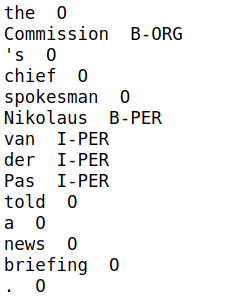
\includegraphics[scale=0.5]{data_print.png}
\end{figure}
如图所示,B-ORG代表的是一个单词,它是一个组织名的开头。
B-PER代表的是一个单词,它是人名的开头,I-PER则代表人名结尾。
o代表其它类型单词,也就是这个单词既不是组织名,也不是地点名同时也不是人名。


我用的数据集是最经典的CoNLL2003命名实体识别数据集,共有九种标签。
\begin{figure}[htp]
   \centering
   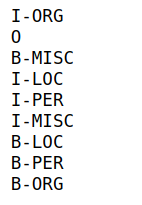
\includegraphics[scale=0.8]{tags.png}
   
\end{figure}


\newpage
\chapter{\sihao\hei 三\quad 模型简介}
{\bfseries 隐马尔科夫模型}

隐马尔科夫模型是可以用于序列标注的一种时序概率图模型,描述的是由一组隐藏
的状态序列(在ner里面就是各个单词对应的标签)生成一个观测序列(就是各个单词)。
序列的每一个位置就是一个时刻。

假设$x_1,x_2,\cdots ,x_n$代表句子中的$n$个单词,$y_1,y_2,\cdots, y_n$就代表这$n$个单词对应的标签。
要计算的是$max(P(y_1,y_2,\cdots, y_n|x_1,x_2,\cdots,x_n))$的概率。HMM通过贝叶斯公式
\[
   P(y_1,y_2,\cdots, y_n|x_1,x_2,\cdots,x_n)=\displaystyle\frac{P(x_1,x_2,\cdots ,x_n|y_1,y_2,\cdots, y_n)P(y_1,y_2,\cdots, y_n)}{P(x_1,x_2,\cdots ,x_n)}
\]
将计算$P(y_1,y_2,\cdots, y_n|x_1,x_2,\cdots,x_n)$改为计算$P(x_1,x_2,\cdots ,x_n|y_1,y_2,\cdots, y_n)P(y_1,y_2,\cdots, y_n)$
。对于$P(x_1,x_2,\cdots ,x_n)$是给定的输入,可以忽略。

HMM有两个基本的假设
\begin{enumerate}
   \item 齐次马尔科夫假设,即当前时刻的状态仅仅依赖于前一个时刻的状态。也就是说$t$时刻第$i$个单词的标签仅仅
依赖于第$i-1$个单词对应的标签。因此$P(y_1,y_2,\cdots, y_n)$可以写成
\[
P(y_1,y_2,\cdots, y_n)=P(y_1)p(y_2|y_1)p(y_3|y_2)\cdots P(y_n|y_{n-1})
\]
   \item 观测独立性假设,即当前时刻的观测仅仅依赖于当前时刻的状态,与其它时刻的状态无关。
   也就是说$t$时刻,单词$i$出现的概率仅仅与它所对应的标签有关,与其它的单词和标签无关。因此
   $P(x_1,x_2,\cdots ,x_n|y_1,y_2,\cdots, y_n)$由观测独立性假设就可以得出
   \[
      P(x_1,x_2,\cdots ,x_n|y_1,y_2,\cdots, y_n)=P(x_1|y_1)P(x_2|y_2)\cdots P(x_n|y_n)
   \]

\end{enumerate}

在HMM中$P(x_i|y_i)$也叫发射概率,意思是在标签为$y_i$的时候,单词$x_i$出现的概率,显然这可以通过训练数据
求出来。$P(y_i|y_{i-1})$也叫转移概率,指的是当前单词被标记为$y_{i-1}$,而它的下一个单词被标记为$y_i$的概率。这两个
概率都可以通过遍历训练数据集中每一个句子以此来统计相应的频数,用频率来代替概率。

从而$P(y_1,y_2,\cdots, y_n|x_1,x_2,\cdots,x_n)$就可以写成$P(x_1|y_1)p(y_1)p(x_2|y_2)p(y_2|y_1)\cdots P(x_n|y_n)P(y_n|y_{n-1})$,
HMM有三个概率矩阵,用$A,B,pi$来表示。这三个矩阵分别记录着状态转移概
率,发射概率以及初始概率。如下图1和图2所示。

\begin{figure}[htp]
   \centering
   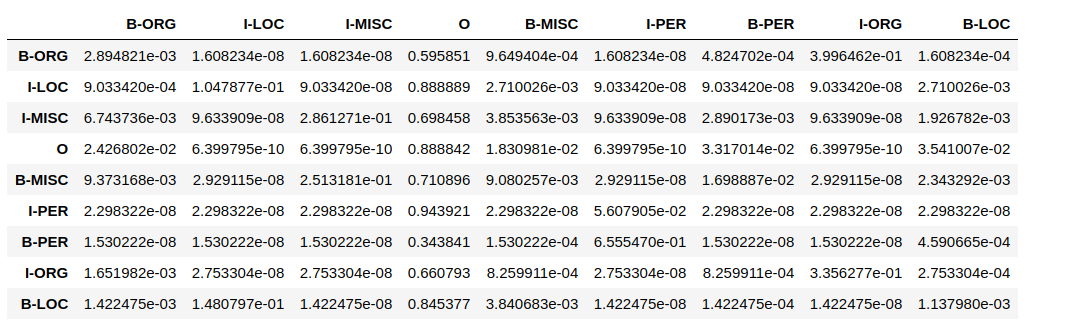
\includegraphics[scale=0.5]{A.png}
   \caption{状态概率转移矩阵}
\end{figure}
这就是每一个标签转移到下一个标签的概率,例如从I-PER转移到O的概率是0.943921。
\begin{figure}[htp]
   \centering
   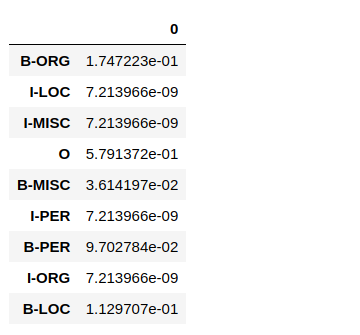
\includegraphics[scale=0.6]{pi.png}
   \caption{初始概率转移矩阵}
\end{figure}
这就是每一种标签的初始概率,例如所有句子的第一个单词是O的概率是0.5791372。
发射概率矩阵比较大就不给出图了,$B[i][j]$的意思就是j这个单词被标记为标签i的概率。
HMM的预测问题通常利用$viterbi$算法,核心思想是最优路径如果通过节点$v_i$,那么从初始节点$v_0$到节点$v_{i-1}$的路径也一定是最优路径。
根据这一思想,就可以不必穷举所有可能的路径再找出概率最大的路径了。只需要从前向后,每一步都是找概率最大的路径上的节点,那么这个节点一定在最优路径上。

现在假设给出这样的句子"Allen Iverson and Michael Jordan are famous basketballer in American"。
首先在发射概率矩阵中找到单词Allen被标记为这九种标签的概率,
分别乘以对应的九种标签的初始概率,
同理找到单词Iverson在发射概率矩阵中的九种概率,用前面的Allen的九种概率分别乘以九种状态转移概率。
例如以I-PER为第一个标签,那么Allen的九种概率分别乘以对应的转移到I-PER的概率(假设Allen被标记为B-PER的概率乘以A[B-PER][I-PER]大于
Allen其他标签的概率乘以相应的转移到I-PER的概率,那么就认为Iverson被标记为I-PER的情况下是从Allen被标记为B-PER转移过来的),
还有其余的九种情况也都要计算出来。由此可见,从第一个单词到第二个单词之间有九种路径,同理
第二个单词到第三个单词也有九种可能的路径(可见如果不是$viterbi$算法的思想,那么每两个单词之间就有81种路径)。
以此类推到最后一个单词American,假设算得American被标记为O的概率最大,而且是从前一个单词in被标记为O的情况
下转移过来的,那么就认为American被标记为O,O就是最优路径上的最后一个节点,前一个节点也是O,以此从后向前推,
就得到了最优路径。下图就是结果
\begin{figure}[htp]
   \centering
   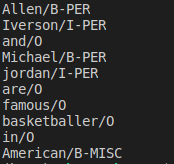
\includegraphics[scale=1.2]{print.png}
   
\end{figure}


{\bfseries 神经网络模型}

最常用的用于序列标注任务的神经网络架构就是BiLSTM-CRF。


\end{document}